\section{Casos de uso.}

En la figura \ref{fig:casosdeuso} podemos ver de forma general el diagrama de casos de usos.

\begin{figure}[htbp]
\centering
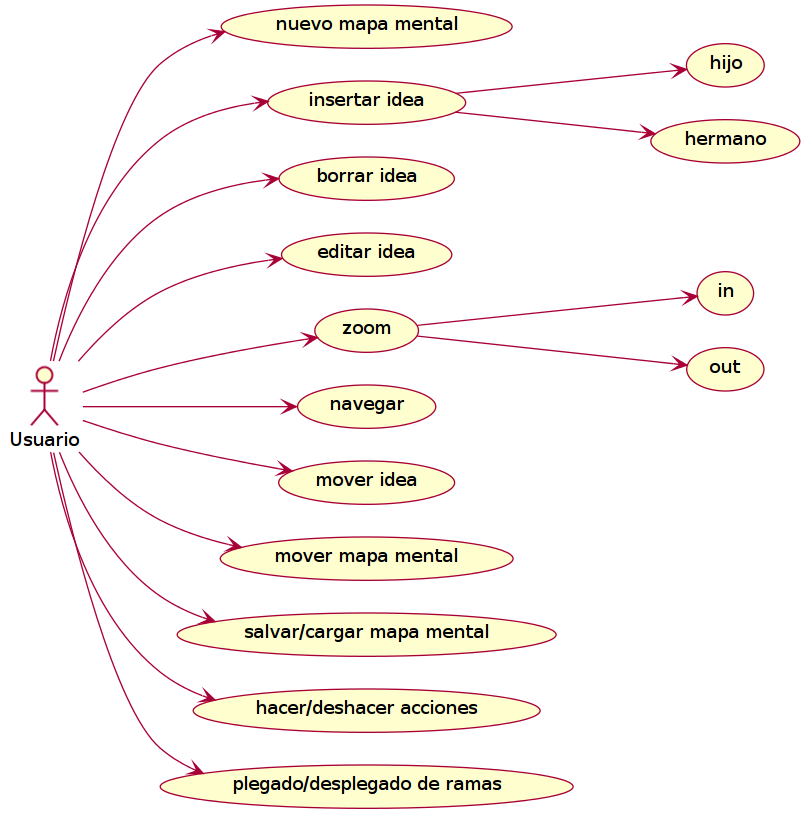
\includegraphics[width=\textwidth]{imagenes/casos-de-uso}
\caption{Casos de uso}
\label{fig:casosdeuso}
\end{figure}

\subsection{Nuevo mapa mental}
El usuario debe de poder reiniciar el editor y empezar un nuevo mapa en cualquier momento. El sistema deberá limpiar la zona de edición eliminando cualquier resto de ediciones anteriores. Una vez borrado se presentará una idea central por defecto que el usuario podrá modificar en todo momento. 

Las acciones que desencadenará esta funcionalidad será un botón y/o la secuencia de teclas $<$Shift+n$>$.

\begin{figure}[tbph]
\centering
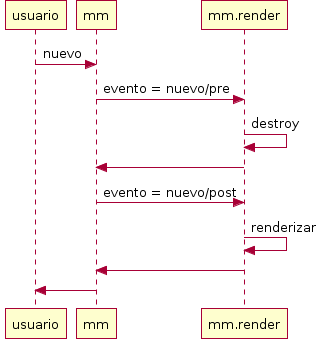
\includegraphics[width=0.4\linewidth]{imagenes/diagrama-seq-nuevo}
\caption{Diagrama de secuencia nuevo}
\label{fig:diagrama-seq-nuevo}
\end{figure}


\subsection{Insertar idea}
Mediante el uso de teclado o ratón el usuario podrá crear nuevas ideas. Esta nueva idea podrá ser tanto hija como hermana de la idea actualmente seleccionada. Debe quedar distribuida en función de los nodos existentes en el mapa mental. 

La secuencia de teclados designadas para la creación de ideas. Son $<$ins$>$ para ideas hijas y $<$Shift+Enter$>$ para crear una idea hermana. 

\begin{figure}[tbph]
\centering
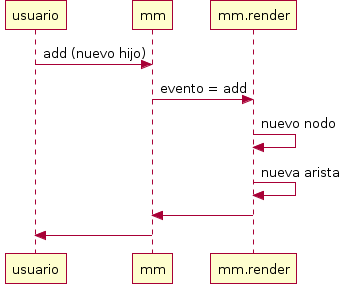
\includegraphics[width=0.4\linewidth]{imagenes/diagrama-seq-add}
\caption{Diagrama de secuencia add}
\label{fig:diagrama-seq-add}
\end{figure}


\subsection{Borrar idea}
Con el teclado ($<$supr$>$) y/o ratón el usuario siempre podrá eliminar un idea del mapa mental. Si existen otras ideas que dependan de la idea a borrar estas también se borrarán. Los nodos se redistribuirán en función de los nodos restantes el mapa mental. 

\begin{figure}[tbph]
\centering
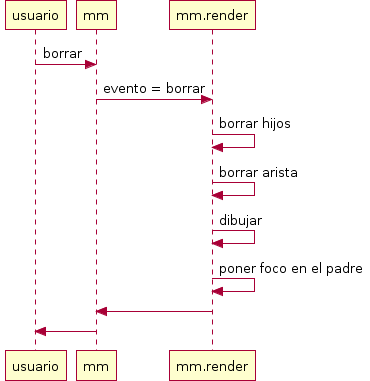
\includegraphics[width=0.4\linewidth]{imagenes/diagrama-seq-borrar}
\caption{Diagrama de secuencia borrar}
\label{fig:diagrama-seq-borrar}
\end{figure}


\subsection{Editar idea}
Toda idea será editable en cualquier momento. El usuario podrá activar el modo de edición y modificar el contenido. Se accederá al modo de edición cuando insertemos, naveguemos, o establezcamos el modo de edición. 

Para entrar y salir del modo de edición se utilizarán las teclas $<$Enter$>$ y $<$Esc$>$ respectivamente. Una vez en modo de edición la secuencias de teclas de la aplicación se ajustarán para que $<$Enter$>$ y $<$Tab$>$ permita salir del modo de edición, con $<$Shift+Enter$>$ se inserte un salto de línea y deshabilite el resto de atajos de teclado. El doble clic y doble touch permitirá entrar en modo de edición.

El editor deberá y ajustándose al tamaño del texto insertado.   

\subsection{Zoom}
La aplicación permitirá acciones de zoom o cambio de escala a la imagen. Ampliar ($<$Ctrl++$>$), reducir ($<$Ctrl+-$>$) y reiniciar la escala ($<$Ctrl+0$>$). Con esta funcionalidad el usuario podrá ajustar las dimensiones del mapa mental a sus necesidades. La rueda del ratón es también una buena opción para realizar zoom in / out.

\begin{figure}[tbph]
\centering
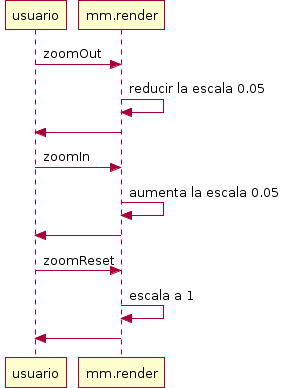
\includegraphics[width=0.4\linewidth]{imagenes/diagrama-seq-zoom}
\caption{Diagrama de secuencia Zoom}
\label{fig:diagrama-seq-zoom}
\end{figure}


\subsection{Navegar}
El usuario debe poder moverse por el mapa mental tanto por teclado como con el ratón o touch. El mapa siempre tendrá una idea activa, o focalizada, que podrá variarse mediante un clic, touch o las siguientes secuencias de tecla:

\begin{itemize}
\item Para ir a la \textbf{idea central} $<$home$>$
\item Para ir a la \textbf{idea padre} de la idea actual $<$left$>$
\item Para ir a la \textbf{idea hija} $<$right$>$
\item Para ir a una \textbf{idea hermana} $<$up$>$ y $<$down$>$
\item Para \textbf{navegar por niveles} podemos utilizar $<$tab$>$
\end{itemize}

\begin{figure}[tbph]
\centering
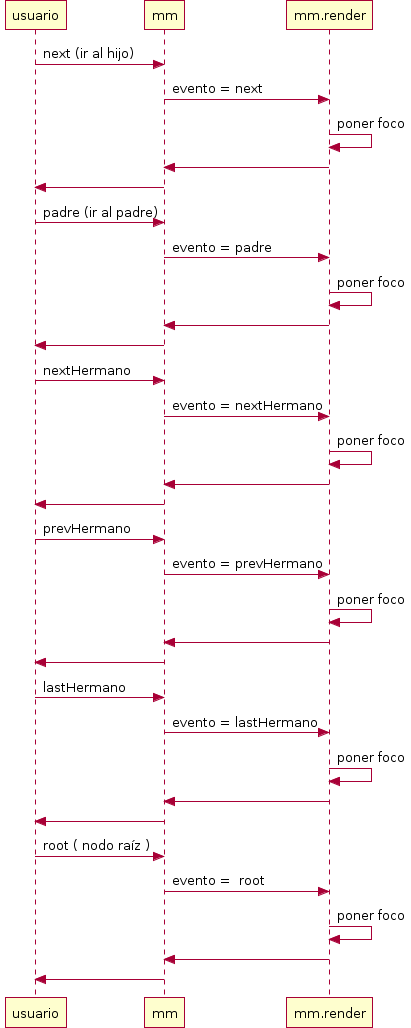
\includegraphics[width=0.4\linewidth]{imagenes/diagrama-seq-navegacion}
\caption{Diagrama de secuencia navegación}
\label{fig:diagrama-seq-navegacion}
\end{figure}


\subsection{Mover idea}
Con el ratón y touch podremos ajustar la posición de los nodos. Desplazando la idea por cualquier punto del marco de visión. 

\subsection{Mover mapa mental}
Con el ratón y touch podremos desplazar el mapa. Ajustar la posición de todo el mapa mental para posibilitar al usuario el marco de visión deseado. 

\subsection{Salvar/cargar mapa mental}
El usuario siempre tendrá opción de salvar y cargar mapas mentales en formato FreeMind. Un formato estándar para que el usuario pueda importar/exportar sus propios mapas mentales o de otros usuarios.

\subsection{Hacer/deshacer acciones}
El sistema dispondrá de opciones típicas de edición como hacer y deshacer. Tantas veces como quiera, en cualquier punto del programa.

\subsection{Plegado/desplegado de ramas}
Las distintas ideas se podrá plegar o desplegar para una mejor visualización. El sistema deberá ajustar las posiciones de las ideas visibles ( que no estén plegada ) al campo de visión siempre que sea posible. 

Para mayor agilidad el programa dispondrá de una secuencia de teclado para plegar ($<$Shift+-$>$) y desplegar ($<$Shift++$>$) además de botones. 

\begin{figure}[tbph]
\centering
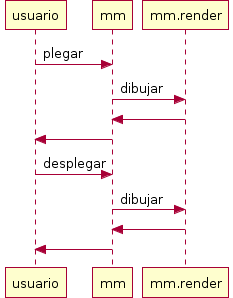
\includegraphics[width=0.3\linewidth]{imagenes/diagrama-seq-plegar}
\caption{Diagrama de secuencia plegar}
\label{fig:diagrama-seq-plegar}
\end{figure}

